\documentclass[12pt,a4paper]{article}
%\usepackage{fontspec, xunicode, xltxtra}  
%\setmainfont{Hiragino Sans GB}  
%\usepackage{xeCJK}
%\setCJKmainfont[BoldFont=STZhongsong, ItalicFont=STKaiti]{STSong}
%\setCJKsansfont[BoldFont=STHeiti]{STXihei}
%\setCJKmonofont{STFangsong}

%使用Xelatex编译

% 设置页面
%==================================================
\linespread{2} %行距
% \usepackage[top=1in,bottom=1in,left=1.25in,right=1.25in]{geometry}
% \headsep=2cm
% \textwidth=16cm \textheight=24.2cm
%==================================================

% 其它需要使用的宏包
%==================================================
\usepackage[colorlinks,linkcolor=blue,anchorcolor=red,citecolor=green,urlcolor=blue]{hyperref} 
\usepackage{tabularx}
\usepackage{authblk}         % 作者信息
\usepackage{algorithm}     % 算法排版
\usepackage{amsmath}     % 数学符号与公式
\usepackage{amsfonts}     % 数学符号与字体
\usepackage{mathrsfs}      % 花体
\usepackage{amssymb}
\usepackage[framemethod=TikZ]{mdframed}

\usepackage{graphicx} 
\usepackage{graphics}
\usepackage{color}
\usepackage{xcolor}
\usepackage{tcolorbox}
\usepackage{lipsum}
\usepackage{empheq}

\usepackage{fancyhdr}       % 设置页眉页脚
\usepackage{fancyvrb}       % 抄录环境
\usepackage{float}              % 管理浮动体
\usepackage{geometry}     % 定制页面格式
\usepackage{hyperref}       % 为PDF文档创建超链接
\usepackage{lineno}          % 生成行号
\usepackage{listings}        % 插入程序源代码
\usepackage{multicol}       % 多栏排版
%\usepackage{natbib}         % 管理文献引用
\usepackage{rotating}       % 旋转文字,图形,表格
\usepackage{subfigure}    % 排版子图形
\usepackage{titlesec}       % 改变章节标题格式
\usepackage{moresize}   % 更多字体大小
\usepackage{anysize}
\usepackage{indentfirst}  % 首段缩进
\usepackage{booktabs}   % 使用\multicolumn
\usepackage{multirow}    % 使用\multirow

\usepackage{wrapfig}
\usepackage{titlesec}     % 改变标题样式
\usepackage{enumitem}
\usepackage{aas_macros}

\newcommand{\myvec}[1]%
   {\stackrel{\raisebox{-2pt}[0pt][0pt]{\small$\rightharpoonup$}}{#1}}  %矢量符号
\renewcommand{\vec}[1]{\boldsymbol{#1}}
\newcommand{\me}{\mathrm{e}}
\newcommand{\mi}{\mathrm{i}}
\newcommand{\dif}{\mathrm{d}}
\newcommand{\tabincell}[2]{\begin{tabular}{@{}#1@{}}#2\end{tabular}}

\def\kpc{{\rm kpc}}
\def\km{{\rm km}}
\def\cm{{\rm cm}}
\def\TeV{{\rm TeV}}
\def\GeV{{\rm GeV}}
\def\MeV{{\rm MeV}}
\def\GV{{\rm GV}}
\def\MV{{\rm MV}}
\def\yr{{\rm yr}}
\def\s{{\rm s}}
\def\ns{{\rm ns}}
\def\GHz{{\rm GHz}}
\def\muGs{{\rm \mu Gs}}
\def\arcsec{{\rm arcsec}}
\def\K{{\rm K}}
\def\microK{\mu{\rm K}}
\def\sr{{\rm sr}}
\newcolumntype{p}{D{,}{\pm}{-1}}

\renewcommand{\figurename}{Fig.}
\renewcommand{\tablename}{Tab.}

\renewcommand{\arraystretch}{1.5}

\setlength{\parindent}{0pt}  %取消每段开头的空格

\newcounter{theo}[section]\setcounter{theo}{0}
\renewcommand{\thetheo}{\arabic{section}.\arabic{theo}}
\newenvironment{theo}[2][]{%
\refstepcounter{theo}%
\ifstrempty{#1}%
{\mdfsetup{%
frametitle={%
\tikz[baseline=(current bounding box.east),outer sep=0pt]
\node[anchor=east,rectangle,fill=blue!20]
{\strut Theorem~\thetheo};}}
}%
{\mdfsetup{%
frametitle={%
\tikz[baseline=(current bounding box.east),outer sep=0pt]
\node[anchor=east,rectangle,fill=blue!20]
{\strut Theorem~\thetheo:~#1};}}%
}%
\mdfsetup{innertopmargin=10pt,linecolor=blue!20,%
linewidth=2pt,topline=true,%
frametitleaboveskip=\dimexpr-\ht\strutbox\relax
}
\begin{mdframed}[]\relax%
\label{#2}}{\end{mdframed}}

\newcommand*\widefbox[1]{\fbox{\hspace{2em}#1\hspace{2em}}}


\title{Turbulence}
\author{}
\date{\today}
\begin{document}

\maketitle

\section{Fully Developed Turbulent Flow}


\subsection{Transition from Laminar to Turbulent Flow}
\cite{munson2009fundamentals, munson2012fundamentals} Flows are classified as laminar or turbulent. For any flow geometry, there is one (or more) dimensionless parameter such that with this parameter value below a particular value the flow is laminar, whereas with the parameter value larger than a certain value the flow is turbulent. The important parameters involved (i.e., Reynolds number, Mach number) and their critical values depend on the specific flow situation involved.

Consider a long section of pipe that is initially filled with a fluid at rest. As the valve is opened to start the flow, the flow velocity and, hence, the Reynolds number increase from zero (no flow) to their maximum steady-state flow values, as shown in Fig. (\ref{fig:Transition}). Assume this transient process is slow enough so that unsteady effects are negligible (quasi-steady flow). For an initial time period the Reynolds number is small enough for laminar flow to occur. At some time the Reynolds number reaches $2100$, and the flow begins its transition to turbulent conditions. Intermittent spots or bursts of turbulence appear. As the Reynolds number is increased, the entire flow field becomes turbulent. The flow remains turbulent as long as the Reynolds number exceeds approximately $4000$.


%===========================================================================================================================
\begin{figure*}
\centering
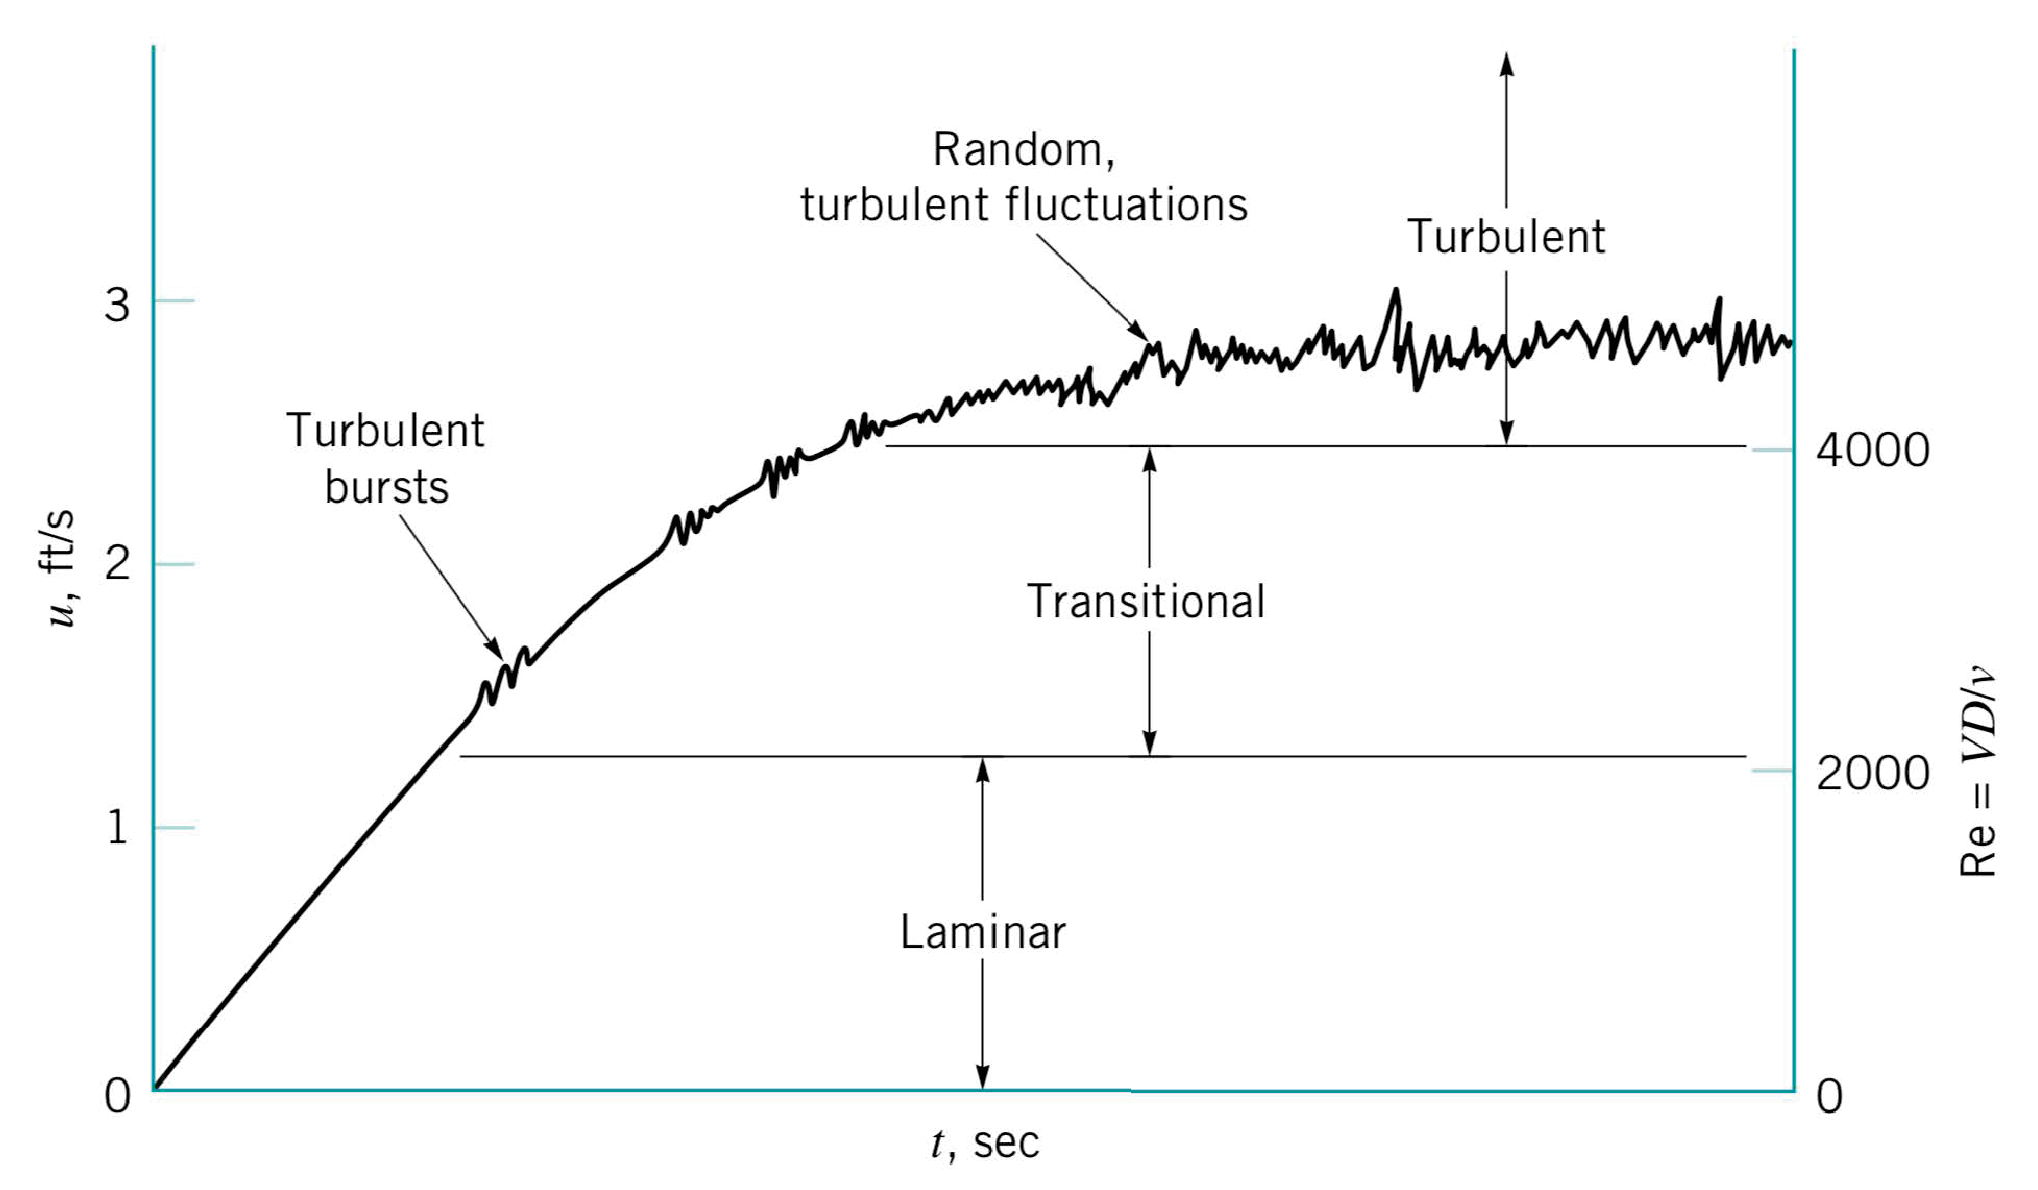
\includegraphics[height=8.cm, angle=0]{Transition.eps}
\caption{
Transition from laminar to turbulent flow in a pipe.
}
\label{fig:Transition}
\end{figure*}
%===========================================================================================================================

A typical trace of the \textcolor{blue}{axial component of velocity} measured at a given location in the flow, $u 􏰔= u(t)$, is shown in Fig. (\ref{axial_velocity}). Its \textcolor{blue}{irregular, random} nature is the distinguishing feature of turbulent flow. The character of many of the important properties of the flow (pressure drop, heat transfer, etc.) depends strongly on the existence and nature of the turbulent fluctuations or randomness indicated. For inviscid flow, the Reynolds number is (strictly speaking) infinite (because the viscosity is zero), and the flow most surely would be turbulent. However, reasonable results were obtained by using the inviscid Bernoulli equation as the governing equation. The reason that such simplified inviscid analyses gave reasonable results is that viscous effects were not very important and the velocity used in the calculations was actually the time-averaged velocity, $\overline{u}$. Calculation of the heat transfer, pressure drop, and many other parameters would not be possible without inclusion of the seemingly small, but very important, effects associated with the randomness of the flow.

%===========================================================================================================================
\begin{figure*}
\centering
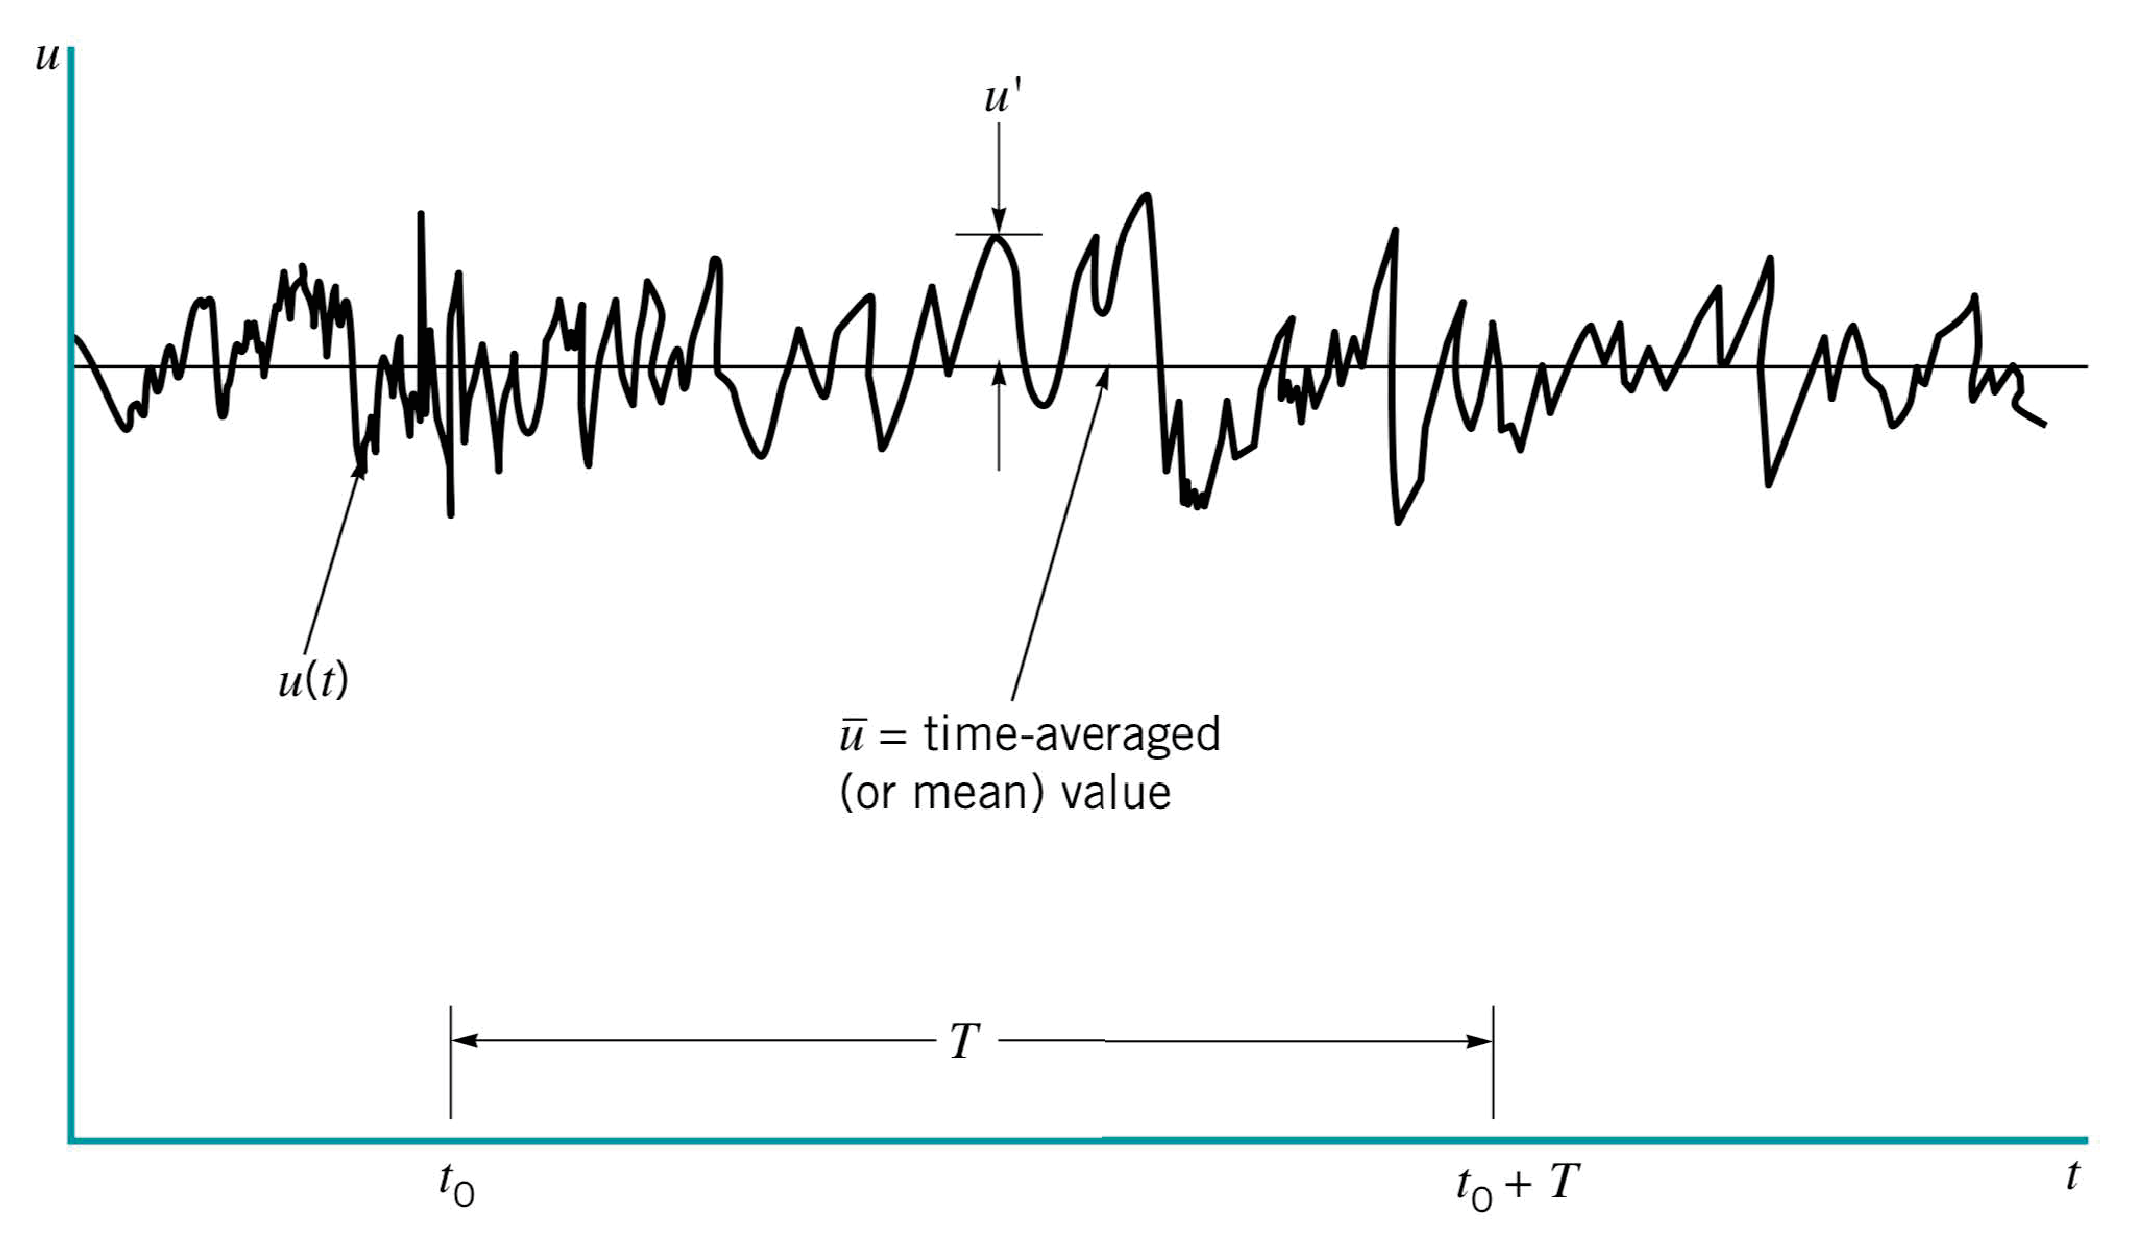
\includegraphics[height=8.cm, angle=0]{axial_velocity.eps}
\caption{
The time-averaged, $\overline{u}$, and fluctuating, $u^\prime$, description of a parameter for turbulent flow.
}
\label{fig:axial_velocity}
\end{figure*}
%===========================================================================================================================

Consider flow in a pan of water placed on a stove. With the stove turned off, the fluid is stationary. The initial sloshing has died out because of viscous dissipation within the water. With the stove turned on, a temperature gradient in the vertical direction, $\partial T/\partial z$, is produced. The water temperature is greatest near the pan bottom and decreases toward the top of the fluid layer. If the temperature difference is very small, the water will remain stationary, even though the water density is smallest near the bottom of the pan because of the decrease in density with an increase in temperature. A further increase in the temperature gradient will cause a buoyancy-driven instability that results in fluid motion - the light, warm water rises to the top, and the heavy, cold water sinks to the bottom. This slow, regular “turning over” increases the heat transfer from the pan to the water and promotes mixing within the pan. As the temperature gradient increases still further, the fluid motion becomes more vigorous and eventually turns into a chaotic, random, turbulent flow with considerable mixing, vaporization (boiling) and greatly increased heat transfer rate. The flow has progressed from a stationary fluid, to laminar flow, and finally to turbulent, multi-phase (liquid and vapor) flow.


Mixing processes and heat and mass transfer processes are considerably enhanced in turbulent flow compared to laminar flow. This is due to the macroscopic scale of the randomness in turbulent flow. We are all familiar with the ``rolling," vigorous eddy type motion of the water in a pan being heated on the stove (even if it is not heated to boiling). Such finite-sized random mixing is very effective in transporting energy and mass throughout the flow field, thereby increasing the various rate processes involved. Laminar flow, on the other hand, can be thought of as very small but finite-sized fluid particles flowing smoothly in layers, one over another. The only randomness and mixing take place on the molecular scale and result in relatively small heat, mass, and momentum transfer rates.


Without turbulence it would be virtually impossible to carry out life as we now know it. Mixing is one positive application of turbulence, as discussed above, but there are other situations where turbulent flow is desirable. To transfer the required heat between a solid and an adjacent fluid (such as in the cooling coils of an air conditioner or a boiler of a power plant) would require an enormously large heat exchanger if the flow were laminar. Similarly, the required mass transfer of a liquid state to a vapor state 1such as is needed in the evaporated cooling system associated with sweating2 would require very large surfaces if the fluid flowing past the surface were laminar rather than turbulent. Turbulence can also aid in delaying flow separation.

Turbulence is also of importance in the mixing of fluids. Smoke from a stack would continue for miles as a ribbon of pollutant without rapid dispersion within the surrounding air if the flow were laminar rather than turbulent. Under certain atmospheric conditions this is observed to occur. Although there is mixing on a molecular scale (laminar flow), it is several orders of magnitude slower and less effective than the mixing on a macroscopic scale (turbulent flow). It is considerably easier to mix cream into a cup of coffee (turbulent flow) than to thoroughly mix two colors of a viscous paint (laminar flow).

In other situations laminar (rather than turbulent) flow is desirable. The pressure drop in pipes (hence, the power requirements for pumping) can be considerably lower if the flow is laminar rather than turbulent. Fortunately, the blood flow through a person's arteries is normally laminar, except in the largest arteries with high blood flowrates. The aerodynamic drag on an airplane wing can be considerably smaller with laminar flow past it than with turbulent flow.


\subsection{Turbulent Shear Stress}
\cite{munson2009fundamentals, munson2012fundamentals} The fundamental difference between laminar and turbulent flow lies in the chaotic, random behavior of the various fluid parameters. Such variations occur in the three components of velocity, the pressure, the shear stress, the temperature, and any other variable that has a field description. Turbulent flow is characterized by random, three-dimensional vorticity (i.e., fluid particle rotation or spin). Such flows can be described in terms of their mean values  on which are superimposed the fluctuations (denoted with a prime). Thus, if $u = u(x, y, z, t)$ is the $x$ component of instantaneous velocity, then its time mean (or time-average) value, $\overline{u}$, is
\begin{equation}
\overline{u} = \dfrac{1}{T} \int_{t_0}^{t_0 +T} u(x, y, z, t) \dif t ~,
\end{equation}
where the time interval, $T$, is considerably longer than the period of the longest fluctuations, but considerably shorter than any unsteadiness of the average velocity.

The fluctuating part of the velocity, $u^\prime$, is that time-varying portion that differs from the average value
\begin{equation}
u = \overline{u} + u^\prime ~, ~~ \text{or} ~~ u^\prime = u - \overline{u} ~.
\end{equation}
the time average of the fluctuations is zero. The fluctuations are equally distributed on either side of the average. Since the square of a fluctuation quantity cannot be negative $[(u^\prime)^2 \geqslant 0]$, its average value is positive. Thus,
\begin{equation}
\overline{(u^\prime)^2} =  \dfrac{1}{T} \int_{t_0}^{t_0 +T} (u^\prime)^2 \dif t  > 0 ~.
\end{equation}
It may be that the average of products of the fluctuations, such as $\overline{u^\prime v^\prime}$, are zero or nonzero (either positive or negative).

The structure and characteristics of turbulence may vary from one flow situation to another. The turbulence intensity, $\mathscr P$, is often defined as the square root of the mean square of the fluctuating velocity divided by the time-averaged velocity, or
\begin{equation}
\mathscr P = \dfrac{\sqrt{\overline{(u^\prime)^2}}}{\overline{u}} = \dfrac{\left[ \dfrac{1}{T} \int_{t_0}^{t_0 +T} (u^\prime)^2 \dif t \right]^{1/2}}{\overline{u}}
\end{equation}
The larger the turbulence intensity, the larger the fluctuations of the velocity (and other flow parameters).

Another turbulence parameter that is different from one flow situation to another is the period of the fluctuations - the time scale of the fluctuations. 

It is tempting to extend the concept of viscous shear stress for laminar flow $(\tau = \mu \dif u/ \dif y)$ to that of turbulent flow by replacing $u$, the instantaneous velocity, by $\overline{u}$, the time-averaged velocity. However, numerous experimental and theoretical studies have shown that such an approach leads to completely incorrect results. That is, $\tau \neq \mu \dif \overline{u}/\dif y$. A physical explanation for this behavior can be found in the concept of what produces a shear stress.

Laminar flow is modeled as fluid particles that flow smoothly along in layers, gliding past the slightly slower or faster ones on either side. The fluid actually consists of numerous molecules darting about in an almost random fashion as is indicated in Fig. (\ref{fig:flow})a. The motion is not entirely random - a slight bias in one direction produces the flowrate we associate with the motion of fluid particles, $\overline{u}$. As the molecules dart across a given plane (plane $A-A$), the ones moving upward have come from an area of smaller average $x$ component of velocity than the ones moving downward, which have come from an area of larger velocity.

The momentum flux in the $x$ direction across plane $A-A$ gives rise to a drag (to the left) of the lower fluid on the upper fluid and an equal but opposite effect of the upper fluid on the lower fluid. The sluggish molecules moving upward across plane $A-A$ must be accelerated by the fluid above this plane. The rate of change of momentum in this process produces (on the macroscopic scale) a shear force. Similarly, the more energetic molecules moving down across plane $A-A$ must be slowed down by the fluid below that plane. This shear force is present only if there is a gradient in $u = u(y)$, otherwise the average $x$ component of velocity (and momentum) of the upward and downward molecules is exactly the same. In addition, there are attractive forces between molecules. By combining these effects we obtain the well-known Newton viscosity law: $\tau = \mu \dif u/\dif y$, where on a molecular basis $\mu$ is related to the mass and speed (temperature) of the random motion of the molecules.

%===========================================================================================================================
\begin{figure*}
\centering
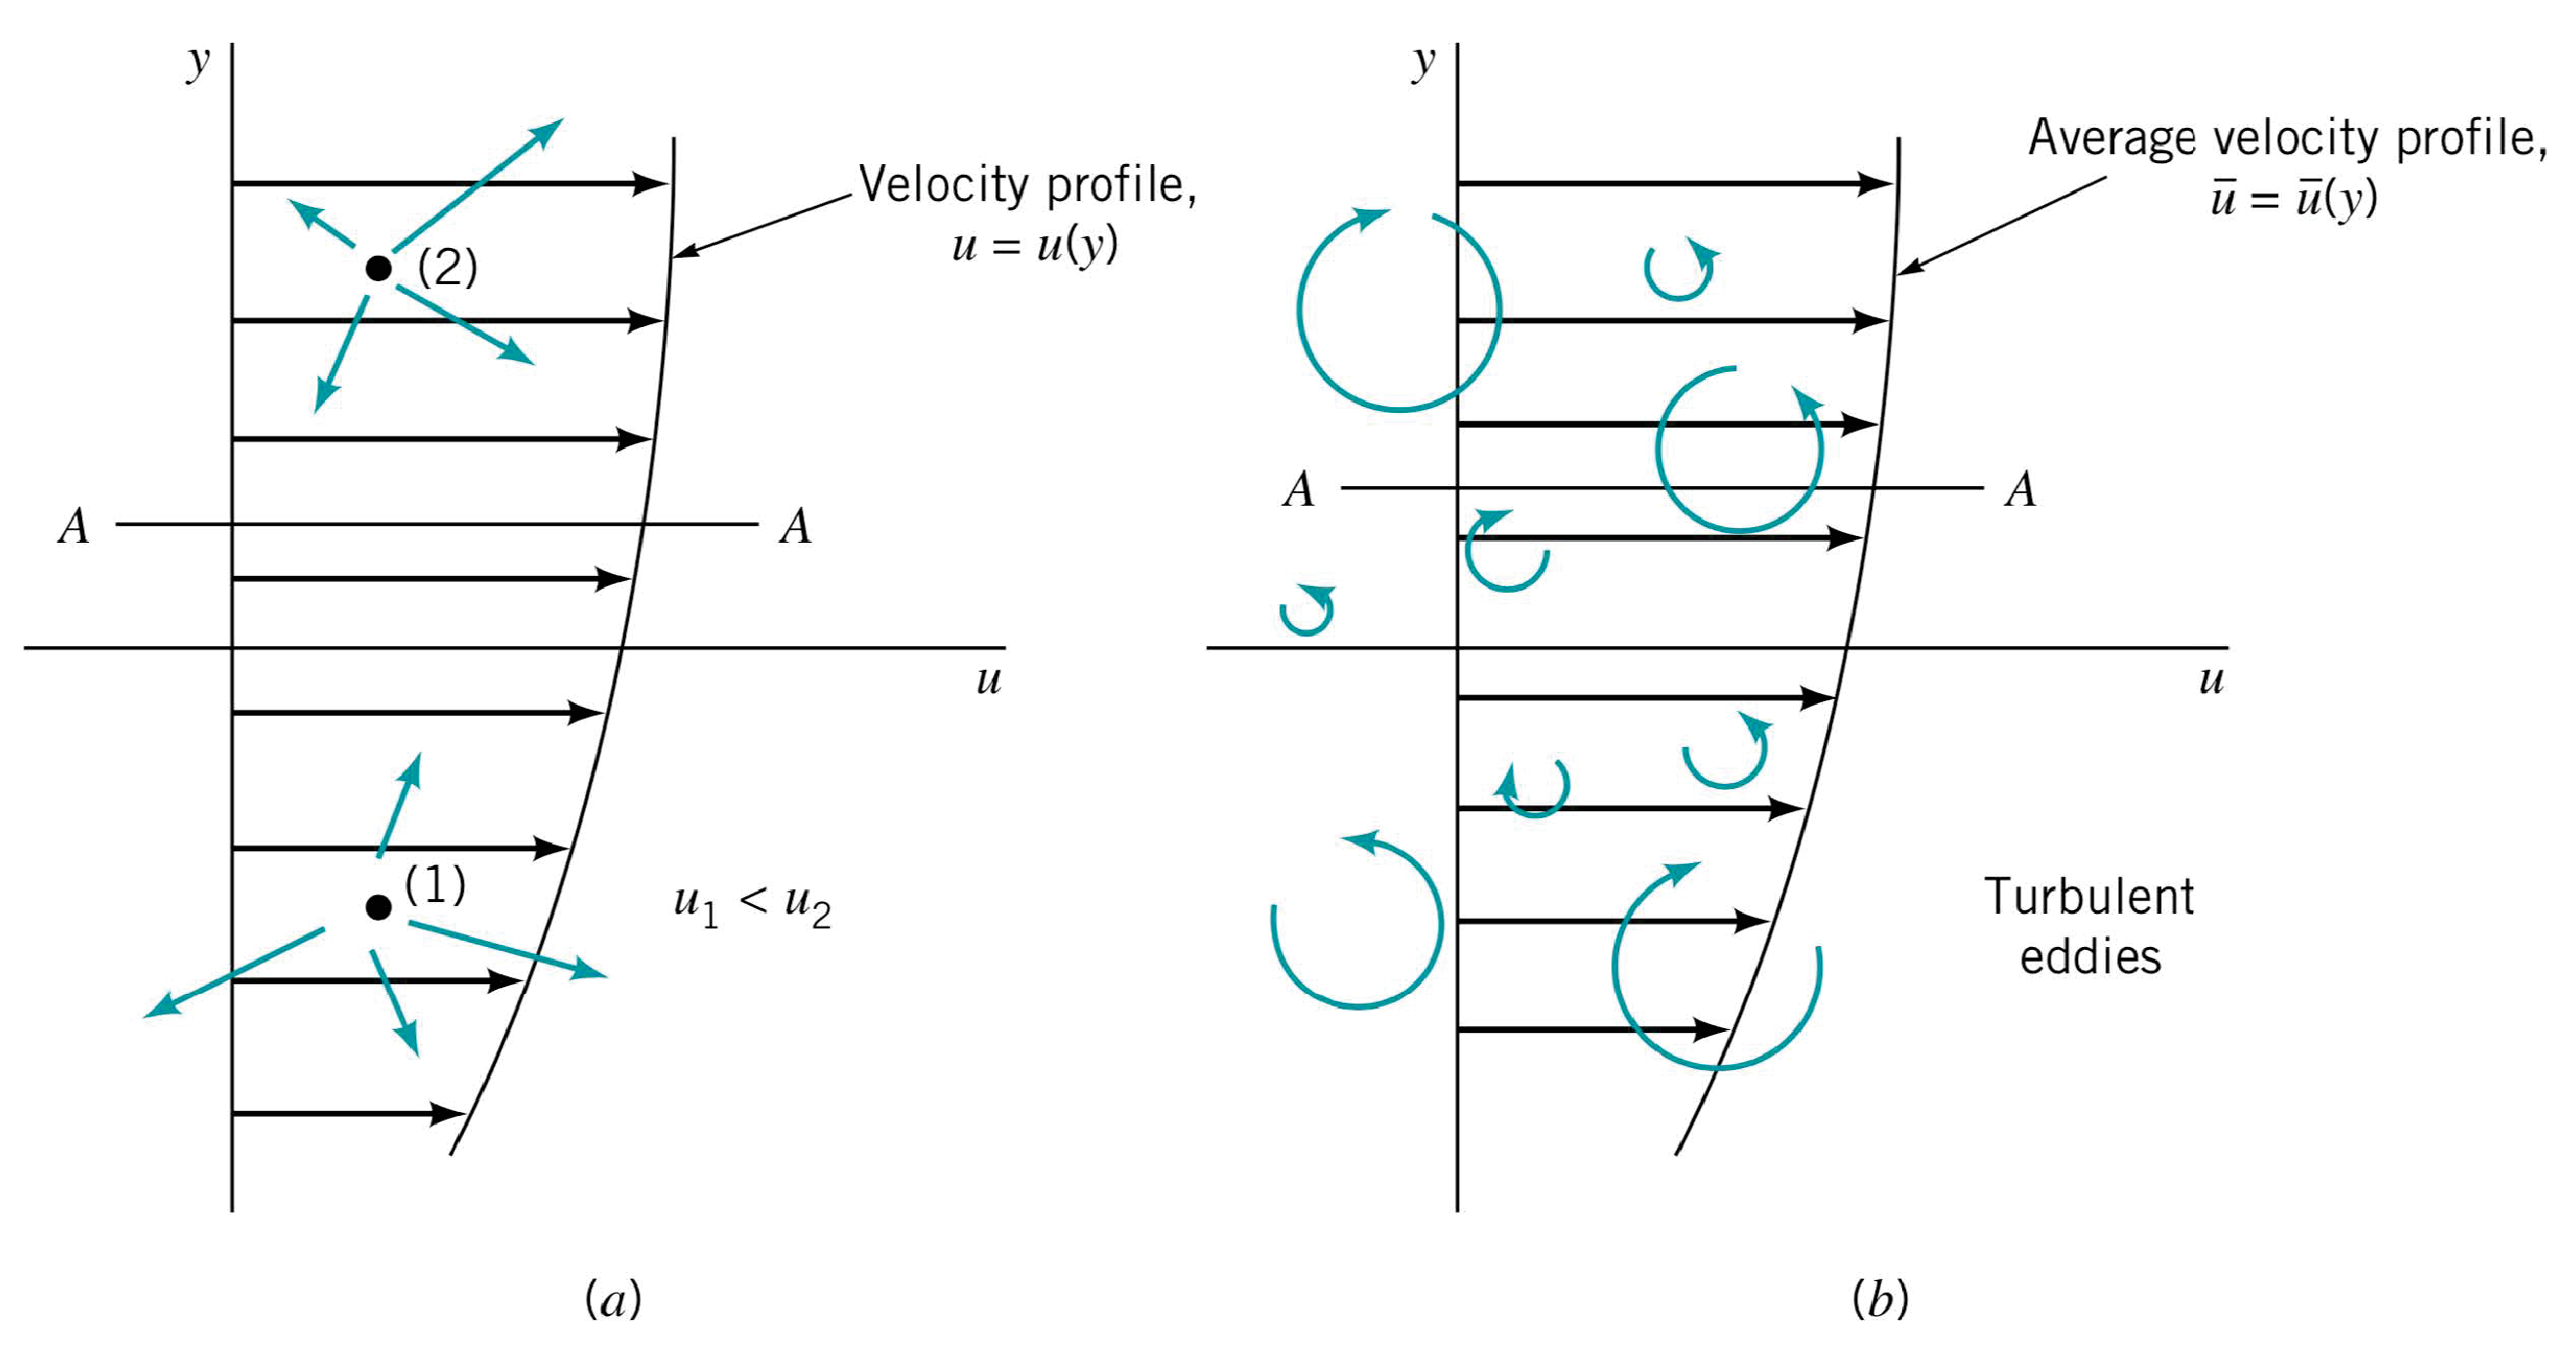
\includegraphics[height=8.cm, angle=0]{flow.eps}
\caption{
(a) Laminar flow shear stress caused by random motion of molecules. (b) Turbulent flow as a series of random, three-dimensional eddies.
}
\label{fig:flow}
\end{figure*}
%===========================================================================================================================

Although the above random motion of the molecules is also present in turbulent flow, there is another factor that is generally more important. A simplistic way of thinking about turbulent flow is to consider it as consisting of a series of random, three-dimensional eddy type motions as is depicted (in one dimension only) in Fig. (\ref{fig:flow})b. These eddies range in size from very small diameter (on the order of the size of a fluid particle) to fairly large diameter (on the order of the size of the object or flow geometry considered). They move about randomly, conveying mass with an average velocity $\overline{u} = \overline{u}(y)$. This eddy structure greatly promotes mixing within the fluid. It also greatly increases the transport of $x$ momentum across plane $A-A$. That is, finite particles of fluid (not merely individual molecules as in laminar flow) are randomly transported across this plane, resulting in a relatively large (when compared with laminar flow) shear force. These particles vary in size but are much larger than molecules.

The random velocity components that account for this momentum transfer (hence, the shear force) are $u^\prime$ (for the $x$ component of velocity) and $v^\prime$ (for the rate of mass transfer crossing the plane). A more detailed consideration of the processes involved will show that the apparent shear stress on plane $A-A$ is given by the following
\begin{equation}
\tau = \mu \dfrac{\dif \overline{u}}{\dif y} - \rho \overline{u^\prime v^\prime} = \tau_{\rm lam} +\tau_{\rm turb} ~.
\end{equation}
If the flow is laminar, $u^\prime = v^\prime = 0$, so that $\overline{u^\prime v^\prime} = 0$ and equation reduces to the customary random molecule-motion-induced laminar shear stress, $\tau_{\rm lam} = \mu \dif \overline{u}/\dif y$. For turbulent flow it is found that the turbulent shear stress, $\tau_{\rm turb} = -\rho \overline{u^\prime v^\prime}$, is positive. Hence, the shear stress is greater in turbulent flow than in laminar flow. Note the units on $\tau_{\rm turb}$ are (density)(velocity)$^2 =􏰔 $(slugs$/$ft$^3$)(ft$/$s)$^2 =$ (slugs $\cdot$ ft$/$s$^2$)/ft$^2$ = lb$/$ft$^2$, or N$/$m$^2$, as expected. Terms of the form 􏰖$-\rho \overline{u^\prime v^\prime}$ (or $-\rho \overline{v^\prime w^\prime}$, etc.) are called \textcolor{red}{Reynolds stresses}.

The shear stress in turbulent flow is not merely proportional to the gradient of the time-averaged velocity, $\overline{u}(y)$. It also contains a contribution due to the random fluctuations of the x and y components of velocity. The density is involved because of the momentum transfer of the fluid within the random eddies. Although the relative magnitude of $\tau_{\rm lam}$ compared to $\tau_{\rm turb}$ is a complex function dependent on the specific flow involved, typical measurements indicate the structure shown in Fig. (\ref{fig:turbulent_flow_in_pipe})a. (the shear stress is proportional to the distance from the centerline of the pipe.) In a very narrow region near the wall (the viscous sublayer), the laminar shear stress is dominant. Away from the wall (in the outer layer) the turbulent portion of the shear stress is dominant. The transition between these two regions occurs in the overlap layer. The corresponding typical velocity profile is shown in Fig. (\ref{fig:turbulent_flow_in_pipe})b.


%===========================================================================================================================
\begin{figure*}
\centering
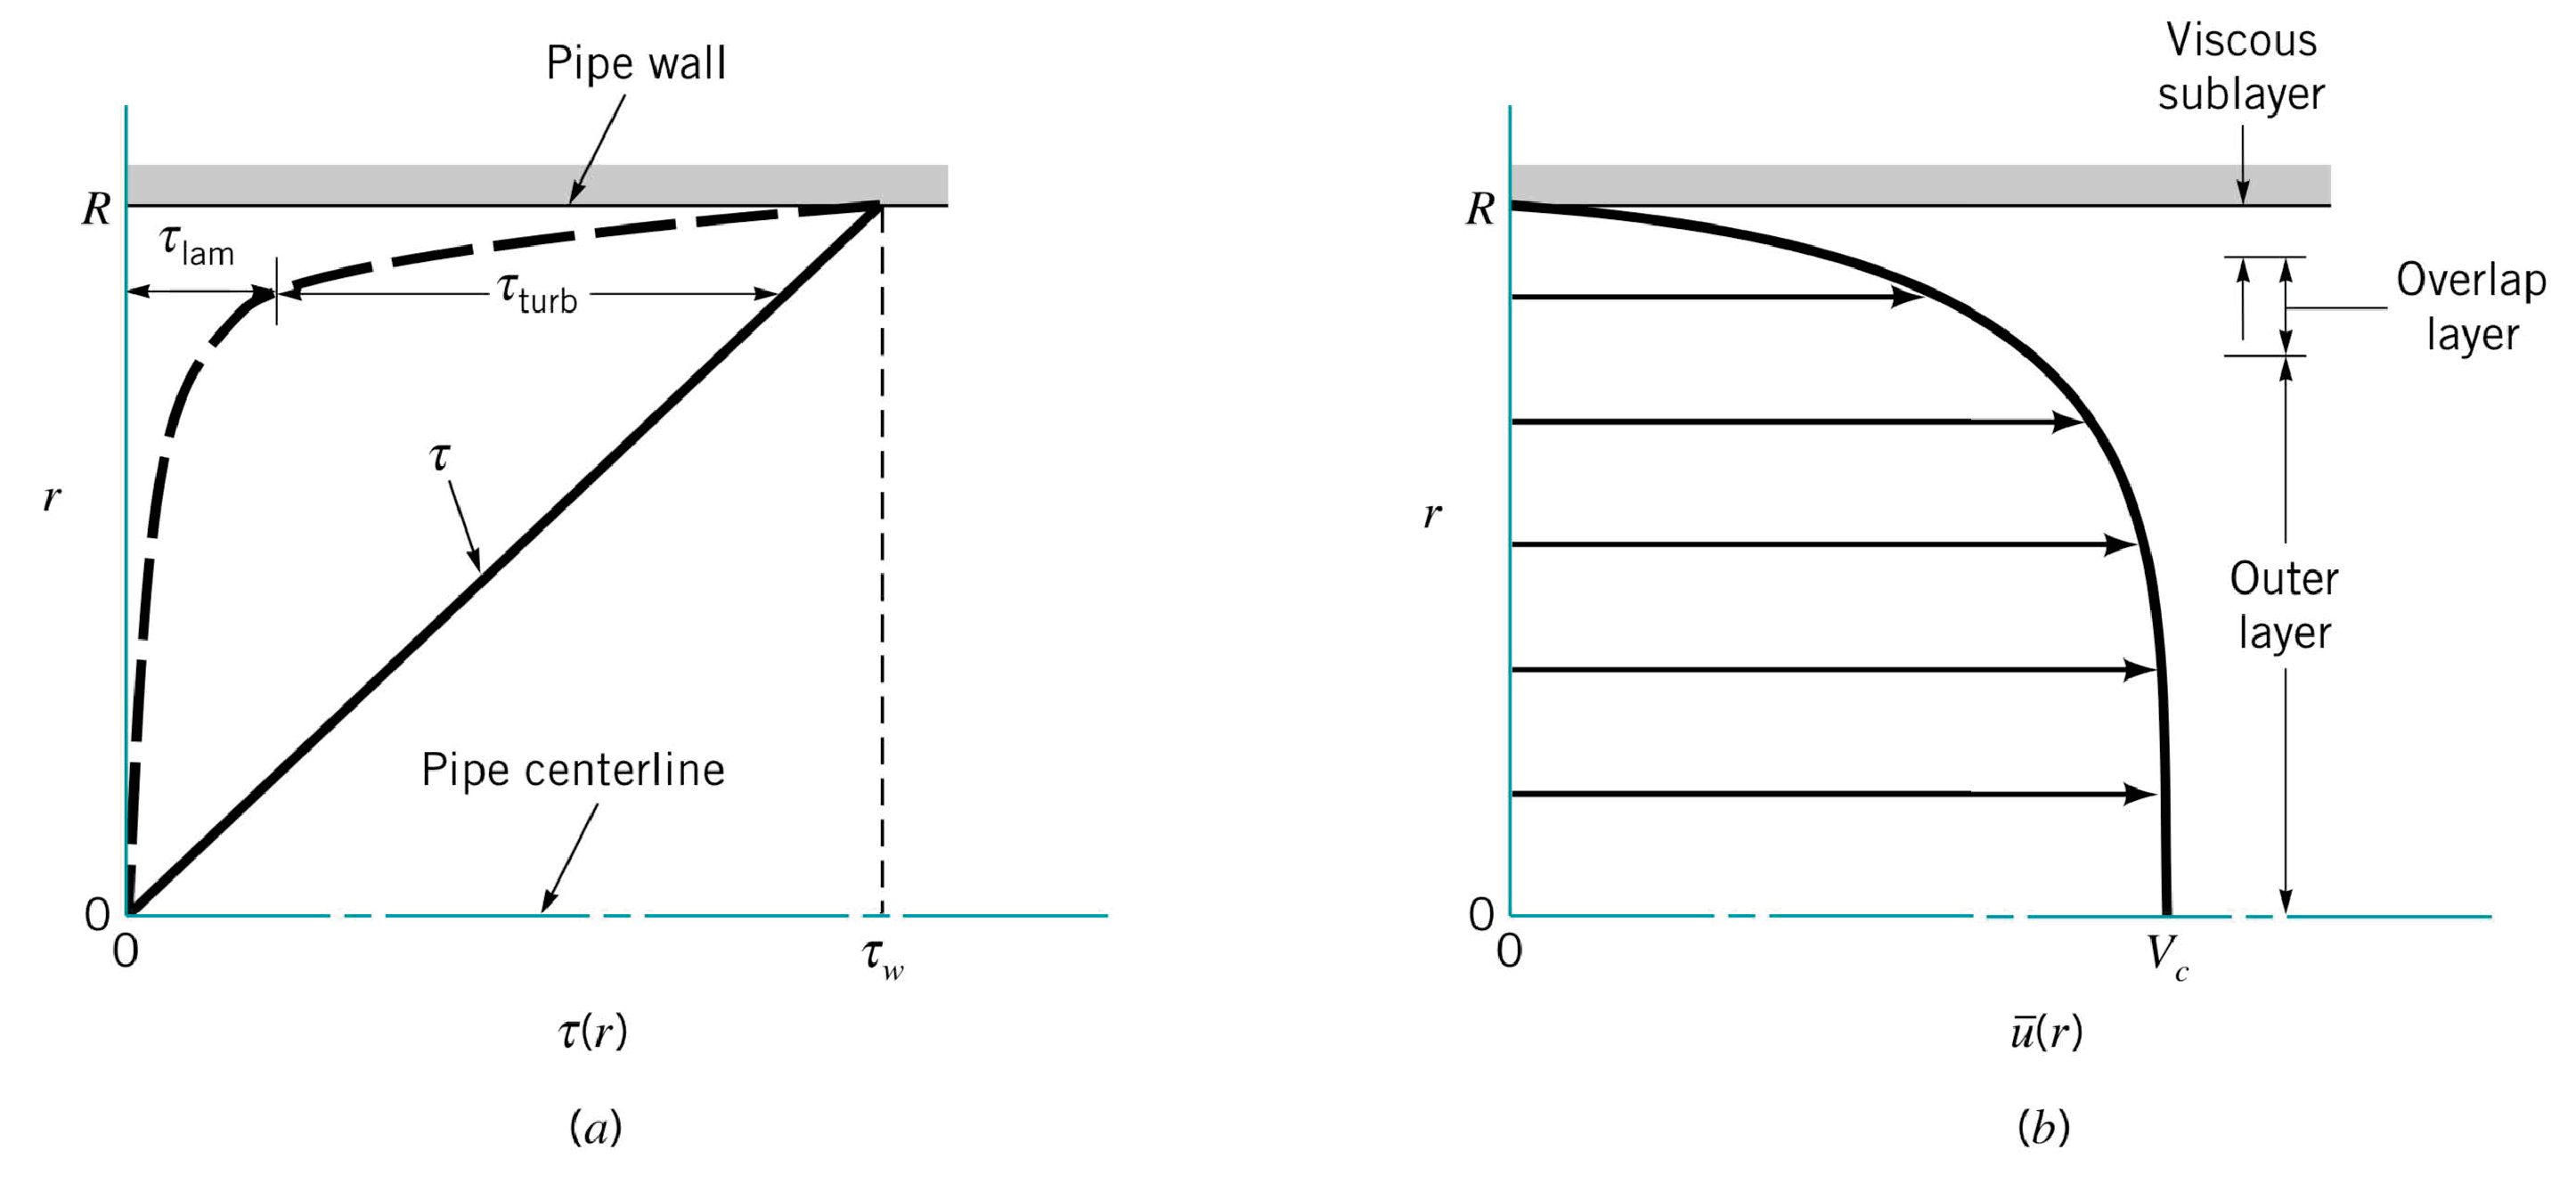
\includegraphics[height=8.cm, angle=0]{turbulent_flow_in_pipe.eps}
\caption{
 Structure of turbulent flow in a pipe. (a) Shear stress. (b) Average velocity.
}
\label{fig:turbulent_flow_in_pipe}
\end{figure*}
%===========================================================================================================================

The scale of the sketches shown in Fig. (\ref{fig:turbulent_flow_in_pipe}) is not necessarily correct. Typically the value of $\tau_{\rm turb}$ is $100$ to $1000$ times greater than $\tau_{\rm lam}$ in the outer region, while the converse is true in the viscous sublayer. A correct modeling of turbulent flow is strongly dependent on an accurate knowledge of $\tau_{\rm turb}$. This, in turn, requires an accurate knowledge of the fluctuations and $u^\prime$ and $v^\prime$, or $\rho \overline{u^\prime v^\prime}$. As yet it is not possible to solve the governing equations 1the Navier-Stokes equations2 for these details of the flow, although numerical techniques  using the largest and fastest computers available have produced important information about some of the characteristics of turbulence.

The vertical scale of Fig. (\ref{fig:turbulent_flow_in_pipe}) is also distorted. The viscous sublayer is usually a very thin layer adjacent to the wall. For example, for water flow in a $3$-in.-diameter pipe with an average velocity of $10$ ft/s, the viscous sublayer is approximately $0.002$ in. thick. Since the fluid motion within this thin layer is critical in terms of the overall flow (the no-slip condition and the wall shear stress occur in this layer), it is not surprising to find that turbulent pipe flow properties can be quite dependent on the roughness of the pipe wall, unlike laminar pipe flow which is independent of roughness. Small roughness elements (scratches, rust, sand or dirt particles, etc.) can easily disturb this viscous sublayer, thereby affecting the entire flow.

An alternate form for the shear stress for turbulent flow is given in terms of the \textcolor{red}{eddy viscosity}, $\eta$, where
\begin{equation}
\tau_{\rm turb} = \eta \dfrac{\dif \overline{u}}{\dif y} ~.
\end{equation}
Unlike the absolute viscosity, $\mu$, which is a known value for a given fluid, the eddy viscosity is a function of both the fluid and the flow conditions. That is, the eddy viscosity of water cannot be looked up in handbooks - its value changes from one turbulent flow condition to another and from one point in a turbulent flow to another.

The inability to accurately determine the Reynolds stress, $\rho \overline{u^\prime v^\prime}$, is equivalent to not knowing the eddy viscosity. The turbulent process could be viewed as the random transport of bundles of fluid particles over a certain distance, $\ell_m$, the \textcolor{red}{mixing length}, from a region of one velocity to another region of a different velocity. By the use of some ad hoc assumptions and physical reasoning, it was concluded that the eddy viscosity was given by
\begin{equation}
\eta = \rho \ell_m^2 \Bigg|  \dfrac{\dif \overline{u}}{\dif y}  \Bigg| ~.
\end{equation}
The turbulent shear stress is
\begin{equation}
\tau_{\rm turb} = \rho \ell_m^2 \left(\dfrac{\dif \overline{u}}{\dif y}  \right)^2 ~.
\end{equation}
The problem is thus to determine the mixing length, $\ell_m$. Further considerations indicate that $\ell_m$ is not a constant throughout the flow field. Near a solid surface the turbulence is dependent on the distance from the surface. Thus, additional assumptions are made regarding how the mixing length varies throughout the flow.

The net result is that as yet there is no general, all-encompassing, useful model that can accurately predict the shear stress throughout a general incompressible, viscous turbulent flow. Without such information it is impossible to integrate the force balance equation to obtain the turbulent velocity profile and other useful information, as was done for laminar flow.

\subsection{Turbulent Velocity Profile}
\cite{munson2009fundamentals, munson2012fundamentals} Considerable information concerning turbulent velocity profiles has been obtained through the use of dimensional analysis, experimentation, numerical simulations, and semiempirical theoretical efforts. In Fig. (\ref{fig:turbulent_flow_in_pipe}), fully developed turbulent flow in a pipe can be broken into three regions which are characterized by their distances from the wall: the viscous sublayer very near the pipe wall, the overlap region, and the outer turbulent layer throughout the center portion of the flow. Within the viscous sublayer the viscous shear stress is dominant compared with the turbulent (or Reynolds) stress, and the random, eddying nature of the flow is essentially absent. In the outer turbulent layer the Reynolds stress is dominant, and there is considerable mixing and randomness to the flow.

The character of the flow within these two regions is entirely different. For example, within the viscous sublayer the fluid viscosity is an important parameter; the density is unimportant. In the outer layer the opposite is true. By a careful use of dimensional analysis arguments for the flow in each layer and by a matching of the results in the common overlap layer, it has been possible to obtain the following conclusions about the turbulent velocity profile in a smooth pipe. 

In the viscous sublayer the velocity profile can be written in dimensionless form as
\begin{equation}
\dfrac{\overline{u}}{u^\ast} = \dfrac{y u^\ast}{v}  ~,
\label{eq:v_linear}
\end{equation}
where $y = R - r$ is the distance measured from the wall, $\overline{u}$ is the time-averaged $x$ component of velocity, and $u^\ast 􏰔= (\tau_w/\rho)^{1/2}$ is termed the \textcolor{red}{friction velocity}. Note that $u^\ast $ is not an actual velocity of the fluid - it is merely a quantity that has dimensions of velocity. As is indicated in Fig. (\ref{fig:velocity_profile_in_pipe}), Eq. (\ref{eq:v_linear}) (commonly called the \textcolor{red}{law of the wall}) is valid very near the smooth wall, for $0 \leqslant yu^\ast /\nu \lesssim 5$.

%===========================================================================================================================
\begin{figure*}
\centering
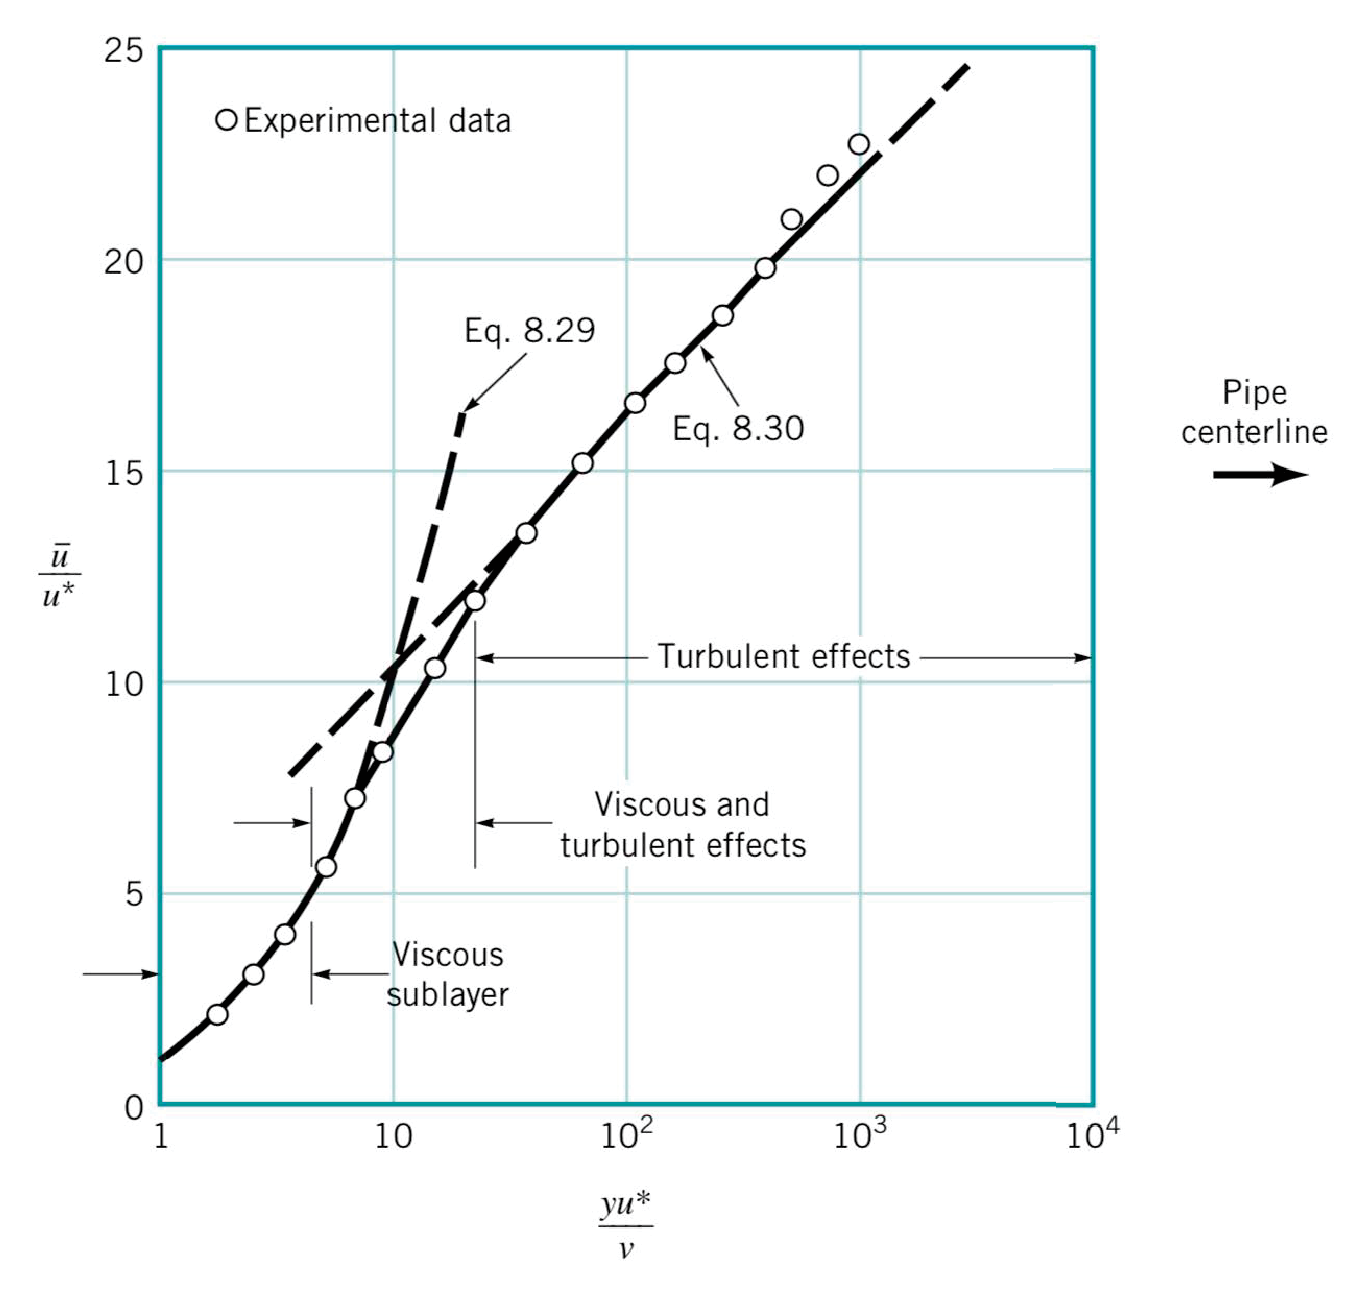
\includegraphics[height=10.cm, angle=0]{velocity_profile_in_pipe.eps}
\caption{
Typical structure of the turbulent velocity profile in a pipe.
}
\label{fig:velocity_profile_in_pipe}
\end{figure*}
%===========================================================================================================================

Dimensional analysis arguments indicate that in the overlap region the velocity should vary as the logarithm of $y$. Thus, the following expression has been proposed:
\begin{equation}
\dfrac{\overline{u}}{u^\ast} = 2.5 \ln\left(  \dfrac{y u^\ast}{v}  \right) + 5.0 ~,
\label{eq:v_log}
\end{equation}
where the constants $2.5$ and $5.0$ have been determined experimentally. As is indicated in Fig. (\ref{fig:velocity_profile_in_pipe}), for regions not too close to the smooth wall, but not all the way out to the pipe center, Eq. (\ref{eq:v_log}) gives a reasonable correlation with the experimental data. Note that the horizontal scale is a logarithmic scale. This tends to exaggerate the size of the viscous sublayer relative to the remainder of the flow. The viscous sublayer is usually quite thin. Similar results can be obtained for turbulent flow past rough walls. 

A number of other correlations exist for the velocity profile in turbulent pipe flow. In the cen- tral region 1the outer turbulent layer2 the expression $(V_c - \overline{u})/u^\ast = 2.5 \ln(R/y)$, where $V_c$ is the centerline velocity, is often suggested as a good correlation with experimental data. Another often-used (and relatively easy to use) correlation is the empirical \textcolor{red}{power-law velocity profile}
\begin{equation}
\dfrac{\overline{u}}{V_c} = \left( 1-\dfrac{r}{R} \right)^{1/n} ~.
\end{equation}
the value of $n$ is a function of the Reynolds number. The one-seventh power-law velocity profile $(n = 7)$ is often used as a reasonable approximation for many practical flows. 

The power-law profile cannot be valid near the wall, since according to this equation the velocity gradient is infinite there. In addition, Equation cannot be precisely valid near the centerline because it does not give $\dif \overline{u}/\dif r = 0$ at $r = 0$. However, it does provide a reasonable approximation to the measured velocity profiles across most of the pipe.

From Fig. (\ref{fig:velocity_profiles}) that the turbulent profiles are much ``flatter" than the laminar profile and that this flatness increases with Reynolds number (i.e., with $n$). The reasonable approximate results are often obtained by using the inviscid Bernoulli equation and by assuming a fictitious uniform velocity profile. Since most flows are turbulent and turbulent flows tend to have nearly uniform velocity profiles, the usefulness of the Bernoulli equation and the uni- form profile assumption is not unexpected. Of course, many properties of the flow cannot be accounted for without including viscous effects.

The turbulent flow characteristics discussed in this section are not unique to turbulent flow in round pipes. Many of the characteristics introduced (i.e., the Reynolds stress, the viscous sublayer, the overlap layer, the outer layer, the general characteristics of the velocity profile, etc.) are found in other turbulent flows. In particular, turbulent pipe flow and turbulent flow past a solid wall (boundary layer flow) share many of these common traits.

%===========================================================================================================================
\begin{figure*}
\centering
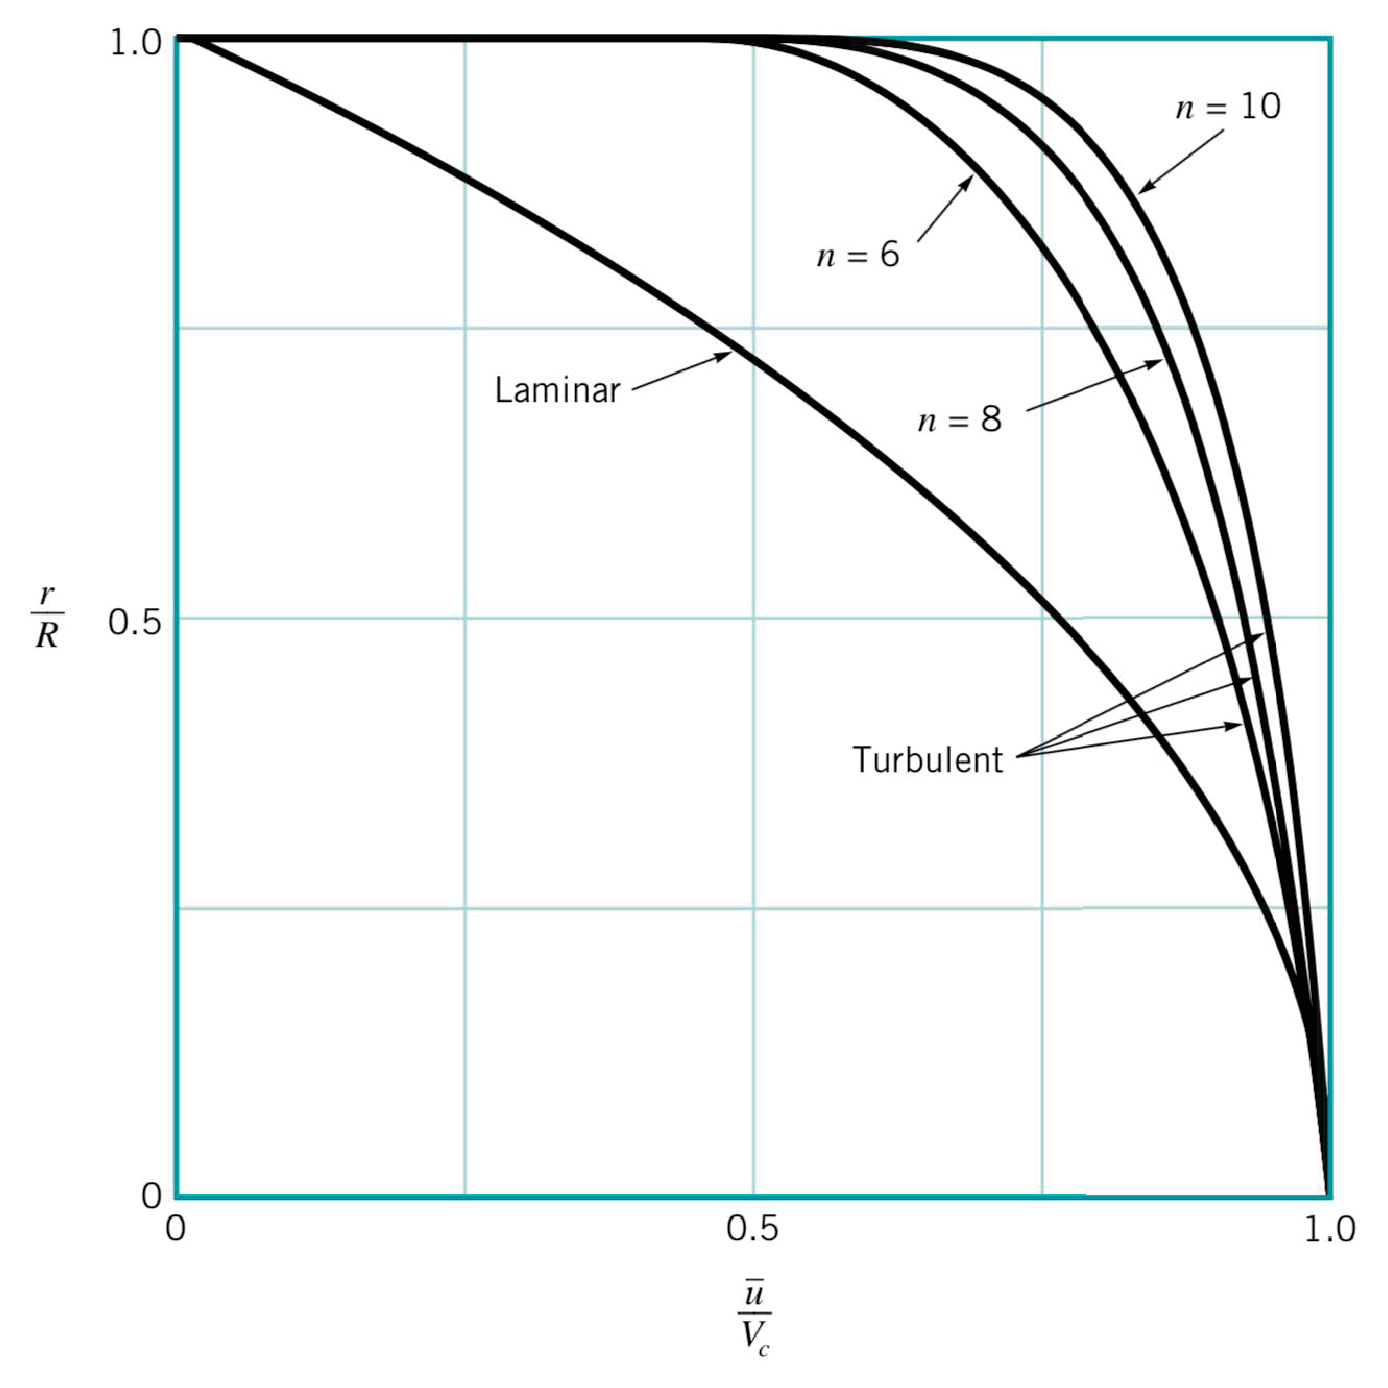
\includegraphics[height=10.cm, angle=0]{velocity_profiles.eps}
\caption{
Typical laminar flow and turbulent flow velocity profiles.
}
\label{fig:velocity_profiles}
\end{figure*}
%===========================================================================================================================







\subsection{Turbulence Modeling}
\cite{munson2009fundamentals, munson2012fundamentals} One can time average the governing Navier-Stokes equations to obtain equations for the average velocity and pressure. However, because the Navier-Stokes equations are nonlinear, the resulting time-averaged differential equations contain not only the desired average pressure and velocity as variables, but also averages of products of the fluctuations - terms of the type that one tried to eliminate by averaging the equations. 

It is not possible to merely average the basic differential equations and obtain governing equations involving only the desired averaged quantities. This is the reason for the variety of ad hoc assumptions that have been proposed to provide ``closure" to the equations governing the average flow. That is, the set of governing equations must be a complete or closed set of equations - the same number of equation as unknowns.

Various attempts have been made to solve this closure problem. Such schemes involving the introduction of an eddy viscosity or the mixing length are termed algebraic or zero-equation models. Other methods include the one-equation model and the two-equation model. These turbulence models are based on the equation for the turbulence kinetic energy and require significant computer usage.


\subsection{Chaos and Turbulence}
\cite{munson2009fundamentals, munson2012fundamentals} Chaos theory involves the behavior of nonlinear dynamical systems and their response to initial and boundary conditions. 

To solve the Navier-Stokes equations for the velocity and pressure fields in a viscous flow, one must specify the particular flow geometry being considered (the boundary conditions) and the condition of the flow at some particular time (the initial conditions). If the Navier-Stokes equations allow chaotic behavior, then the state of the flow at times after the initial time may be very, very sensitive to the initial conditions. A slight variation to the initial flow conditions may cause the flow at later times to be quite different than it would have been with the original, only slightly different initial conditions. When carried to the extreme, the flow may be ``chaotic," ``random," or perhaps ``turbulent."

The occurrence of such behavior would depend on the value of the \textcolor{orange}{Reynolds number}. It may be found that for sufficiently small Reynolds numbers the flow is not chaotic (i.e., it is laminar), while for large Reynolds numbers it is chaotic with turbulent characteristics.






































%%%%%%%%%%%%%%%%%%%%%%%%%%%%%%%%%%%%%%%%%%%%%%%%%%%%%%%%%%%%%%%%%%%%%%
\bibliographystyle{unsrt_update}
\bibliography{ref}
%%%%%%%%%%%%%%%%%%%%%%%%%%%%%%%%%%%%%%%%%%%%%%%%%%%%%%%%%%%%%%%%%%%%%%

\end{document}